\documentclass[tikz]{standalone}

\usepackage{fontspec}

\usetikzlibrary{arrows}
\usetikzlibrary{calc}
\usetikzlibrary{decorations.pathreplacing}
\usetikzlibrary{positioning}
\usetikzlibrary{matrix}

\usepackage{fontspec}

\begin{document}

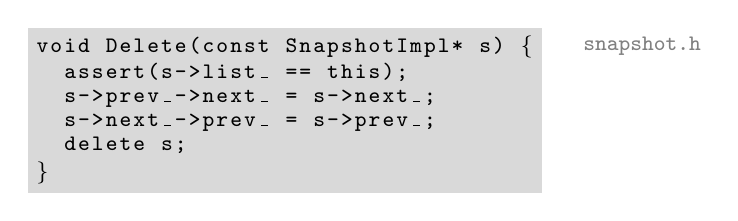
\begin{tikzpicture}
  [node distance=5mm, >=stealth',
  every node/.style={font=\footnotesize},
  every matrix/.style={fill=black!15, inner sep=1mm, row sep=0.5mm,
                        matrix of nodes, nodes in empty cells,
                        minimum height=0.5em, minimum width=.5em,
                        nodes={anchor=base, inner sep=0, font=\ttfamily\footnotesize}}]

  \matrix (snippet) {
v & o & i & d &   & D & e & l & e & t & e & ( & c & o & n & s & t &   & S & n & a & p & s & h & o & t & I & m & p & l & * &   & s & ) &   & \{ \\
  &   & a & s & s & e & r & t & ( & s & - & > & l & i & s & t & \_ &   & = & = &   & t & h & i & s & ) & ; &   &   &   &   &   &   &   &   &   \\
  &   & s & - & > & p & r & e & v & \_ & - & > & n & e & x & t & \_ &   & = &   & s & - & > & n & e & x & t & \_ & ; &   &   &   &   &   &   &   \\
  &   & s & - & > & n & e & x & t & \_ & - & > & p & r & e & v & \_ &   & = &   & s & - & > & p & r & e & v & \_ & ; &   &   &   &   &   &   &   \\
  &   & d & e & l & e & t & e &   & s & ; &   &   &   &   &   &   &   &   &   &   &   &   &   &   &   &   &   &   &   &   &   &   &   &   &   \\
\} &   &   &   &   &   &   &   &   &   &   &   &   &   &   &   &   &   &   &   &   &   &   &   &   &   &   &   &   &   &   &   &   &   &   &   \\
  };


 \node [above, anchor=west, black!50, xshift=0.5cm]
        at (snippet-1-36.east)
        {\texttt{snapshot.h}};
\end{tikzpicture}

\end{document}
